\documentclass[a4paper, 12pt]{report}

%%%%%%%%%%%%
% Packages %
%%%%%%%%%%%%

\usepackage[english]{babel}
\usepackage[noheader]{packages/sleek}
\usepackage{packages/sleek-title}
\usepackage{packages/sleek-theorems}
\usepackage{packages/sleek-listings}
\usepackage{packages/seg-report-extra}
\usepackage{longtable}

\newcommand{\defaultInstructions}{
\begin{instructions}
Please remove all expectations and assessment environments from this page before submitting, including this instruction.  This is placeholder content to help you write the report.  It must not be included in the final report.
\end{instructions}
}

%%%%%%%%%%%%%%
% Title-page %
%%%%%%%%%%%%%%

\logo{./resources/pdf/Kcl-logo.pdf}
%\institute{Random University}
\faculty{Faculty of Natural, Mathematical, and Engineering Sciences}
\department{Department of Informatics}
\title{Software Engineering Group Project}
\subtitle{Virtual Study Room}%%% Insert project name here
\author{\textit{Team MangoCat}\\   %%% Add team name here
Aamukta Malyada Thogata\\                        %%% Add first author here
Agrima Khare\\                        %%% Add second author here
Isha Selvakumaran\\                      %%% Add three author here
Natalia Ahsan\\                       %%% Add four author here
Onessa Crispeyn\\                       %%% Add five author here
Prapti Patel\\                        %%% Add six author here
Yonna Khatri\\                      %%% Add seven author here
Yuliia Bohakt\\                      %%% Add eight author here
}
\date{\today}

%%%%%%%%%%%%%%%%
% Bibliography %
%%%%%%%%%%%%%%%%

\addbibresource{./resources/bib/references.bib}

%%%%%%%%%%
% Others %
%%%%%%%%%%

\lstdefinestyle{latex}{
    language=TeX,
    style=default,
    %%%%%
    commentstyle=\ForestGreen,
    keywordstyle=\TrueBlue,
    stringstyle=\VeronicaPurple,
    emphstyle=\TrueBlue,
    %%%%%
    emph={LaTeX, usepackage, textit, textbf, textsc}
}

\FrameTBStyle{latex}

\def\tbs{\textbackslash}

%%%%%%%%%%%%
% Document %
%%%%%%%%%%%%

\begin{document}
    \maketitle
    \romantableofcontents

    \chapter{Introduction}
\label{chap:introduction}

\defaultInstructions

\begin{expectations}
A good introduction gives the reader a good idea of what the project is about in the shortest amount of text.  A reader should be able to get through this chapter very quickly and decide whether this project is relevant to their interests.
\begin{itemize}
\item A summary of the overriding business objective of the application.  Explain what the client, the end-users of your application, or the organisation deploying it would gain from the application.  Explain this value from the perspective of the client's or users' world, not from your perspective as a developer.   Do not list features, requirements, or specifications here.  The software is a means to an end, not the objective in itself.
\item A statement of the type of system you built, including the platforms on which it can be used, and the technology stack used to build it.
\end{itemize}
This chapter does not require any sections of subsections.  In many projects, two short paragraphs will be enough.  However, you can use more if the objective cannot be explained in a single paragraph.  Note, though, that you will be developing the objectives further in the next chapter.

\end{expectations}

\begin{length}
A single page should be sufficient for this chapter.  More than two pages is too long.
\end{length}

 Our project ‘The Study Spot’ is a virtual study space that students can use to study together with friends.
Our primary goal is to enhance student productivity and collaboration by providing features such as creating virtual study rooms, easy sharing of documents, chat rooms, rewards and shared to-do lists.

By fostering an interactive and organised study environment, our application will help users maintain focus and subsequently enhance their learning experience.

The end-users - students - will gain from improved time management, healthy competition and access to a shared study environment, making their study sessions more efficient and enjoyable.
    \chapter{Objectives and stakeholders}
\label{sect:objectives}

\defaultInstructions

\begin{length}
There are no strict length requirements for this chapter.  However, it is important that the writing is clear and concise.  Avoid repeating yourself.  It is expected that a typical project needs 1--3 pages, but this can vary considerably from project to project.
\end{length}

\begin{expectations}
This is a short chapter that identifies the objectives and stakeholders of the project.  A good report also discusses how the different types of stakeholder are affected by the project or how they could be affected by the project.

As you explain the project objectives, focus exclusively on what value the system adds to the stakeholders.  Your objectives should justify \emph{why} you are building the system.  The software requirements are \emph{not} objectives.  The software requirements explain \emph{what} your system can do.  In other words, they are a way to achieve objectives.  Software requirements do \emph{not} belong in this chapter.  Your project should have at least one objective.  Otherwise, the project is a pointless exercise.  Many objectives do not necessarily make for a better project.

Some stakeholders of a project will be obvious: e.g. the people who the beneficiaries of the value your project adds.  However, it is important to be aware of all stakeholders.  The stakeholder D.A.N.C.E. tool to identify all stakeholders and it is explained in a video on project initiation.  Consider carefully how each stakeholder is affected by your project and who the key stakeholders are.

The section headers below provide a suggested structure.  You should feel free to change it or extend it.
\end{expectations}

\section{Project objectives}
\label{sect:objectives}

\section{Stakeholder}
\label{sect:stakeholder}
\begin{length}
    Students (Primary Stakeholders)
        Impact: Benefit directly from improved academic performance, enhanced subject understanding, and increased motivation through collaborative learning.
        Age Group: The platform accommodates students across all educational stages, from school to university level.
    Platform Developers and Administrators
        Impact: Responsible for maintaining website functionality, ensuring data security, and improving user experience. Their work directly affects user satisfaction and engagement.
\end{length}

\subsection{Stakeholder analysis}
\subsection{Key stakeholders}
\begin{length}
    The project's success relies on meeting the needs of each stakeholder group. By focusing on students as the primary users, the platform has been designed to be intuitive and engaging. Furthermore, feedback loops from these users will prove essential for continuous improvement. This systematic approach to identifying objectives and understanding stakeholder impact ensures the project remains both user-focused and goal-oriented.
\end{length}
    \chapter{Specifications}
\label{chap:specifications}

\defaultInstructions

\begin{length}
There are no strict length requirements for this chapter.  However, it is important that the writing is clear and concise.  Avoid repeating yourself.  It is expected that a typical project needs 1--5 pages, but this can vary considerably from project to project.
\end{length}

\begin{expectations}
This chapter should provide the specifications of the software that you have implemented.  Good specifications are clear, concise, consistent (with one another and with the project objectives), estimable (the effort required of functional requirements should be estimable), and testable (you should be able to create automated or manual tests for these specifications).

A significant part of this chapter covers functional requirements/specifications.  These refer to the product features your team has developed.  Present a clear overview of all functional requirements/specifications that can be found in the deployed system.  For each feature, explain how it contributes to the project objectives, and explain how/where it can be found.  Do \emph{not} mix the specifications the team managed to implement with those they did not.  

If necessary or helpful for clarity, explain what is out of scope of the project in a distinct section.  You may discuss ideas for functional specifications the team did not manage to implement, provided this discussion is clearly distinct from the project's achieved functional specifications.

The project objectives will also entail certain non-functional specifications.  These may include, for example, reliability, usability, portability, scalability, performance, compatibility, security, compliance, etc.  Identify which non-functional specifications are important to this project and define them.  Make sure to present them in order of importance, and relate each one to the project objectives.  

The section headers below provide a suggested structure.  You should feel free to change it or extend it.
\end{expectations}

\section{Functional specifications}
\label{sect:functional-specifications}

\section{Non-functional specifications}
\label{sect:non-functional-specifications}

    \chapter{Project management}
\label{chap:project-management}

In order to manage this project, we split up administrative tasks between the members of the team to ensure that everyone had a role in management and keeping track of the project. We did this so all members had some responsibility and could ensure accountability throughout the project. This also improved efficiency as other members knew who to look to when needing help with a certain task and prevented all the load from being put onto one individual. We split up the roles as follows:

\begin{itemize}
    \item \textbf{Chair of Meetings and Organiser} - Aamukta Thogata
    \item \textbf{Trello Board} - Prapti Patel
    \item \textbf{GitHub Repo} - Yonna Khatri
    \item \textbf{Wellbeing Manager} - Onessa Crispeyn
    \item \textbf{Report} - Isha Selvakumaran
    \item \textbf{Deployment} - Yuliia Bohak
    \item \textbf{Meeting Scheduling} - Natalia Ahsan
    \item \textbf{Meeting Notes} - Agrima Khare
\end{itemize}

For the duration of the project, we kept logs and records of all meetings and all decisions made on Notion and Team Feedback. We planned a rough timeline for the project in the first week and prioritised the features to ensure that we could complete the most important features on time. 

As a team, we spent a lot of time planning and brainstorming before moving on to development ( mostly during winter break ) to ensure that we all had a clear vision of what we wanted the project to be and to ensure that we were all on the same page. This was very important to us as we noticed from previous projects that members having different visions can cause problems later on and disagreements or tasks being completed but then becoming redundant.

Before starting coding, we also made sure to decide on a good tech stack. We decided to keep using Django for the backend as it was something we were all familiar with after the small group project, and this would enable us to make a good start on the backend in the early weeks. We used this to our advantage and focused on learning React for the frontend as a team during the first few weeks while clearing out most of the easier backend tasks using Django. This proved well for our team as it gave us time to learn something new without having to sacrifice many weeks without actually coding.

We set expectations for the workload and how much we would aim to contribute early on and decided when we would meet each week and have kept this consistent over the last 3 months. Due to this, we have all been able to stick to deadlines and have had very few issues with tasks running over or not being completed.

The use of our Trello here to assign weekly tasks aligns with principles from Kanban, allowing us to visualize tasks. However, as the project progressed, we shifted towards a more Agile approach, focusing on iterative improvements.

We also went over some rules which we laid down to ensure that the project development would go smoothly. This included rules such as :

\begin{itemize}
    \item We would only push a feature to \texttt{main} \textbf{after} all tests had been written and were fully passing.
    \item We would not ask each other to complete a task in under 48 hours of it being assigned, to be respectful of each other's time.
    \item We would make sure that where we could, our code was fully commented and had guidelines to help others understand.
    \item For larger features, we would wait until a team meeting to approve a pull request so the team could review the changes.
\end{itemize}


Although we kept to our ground rules as much as possible, at times, it was necessary to go down a different route and times when they would not have worked out:

\begin{itemize}
    \item Though we all followed our roles for the most part, we sometimes made some changes. For example:
    \begin{itemize}
        \item A number of us worked on deployment as it was not feasible for one person to take on the whole task.
    \end{itemize}
    \item We would not move Trello tasks punctually at times, and towards the end of the project, other methods of task tracking were also used.  
    So, while our initial approach to project tracking with Trello was effective in the early stages, it became less practical towards the end. 
    \item As more and more small changes were being made, pull requests became more frequent, and it was not convenient to have to wait until a meeting to merge them.
\end{itemize}

These experiences showed us the importance of adapting our project management tools and strategies as the project evolved, as what worked with one part of the project might not work throughout.

Over the course of the last three months, we also did have some issues.

\begin{itemize}
    \item \textbf{Issues with deployment} and having to switch to Vercel and Render from PythonAnywhere. This was one of our most critical decisions and, although it caused significant delays initially, it proved to be a more stable and necessary decision.
    \item \textbf{Issues with Spotify Premium} and needing to add free music.
    \item \textbf{Issues with login}, requiring us to allow only one login per browser to avoid authentication token conflicts.
    \item \textbf{Calendar feature taking a lot longer than expected}, but ultimately becoming a much bigger and more useful feature.
    \item \textbf{Website design evolving over time}, especially after receiving feedback from the advisor.
\end{itemize}
    \chapter{Design and implementation}
\label{chap:design-and-implementation}

\section{Architecture}
\label{sect:architecture}

Since our main stakeholders are students, we decided to base our design decisions on what would attract students to our website. Our colour palette was decided early on, and we focused on a gender neutral, yet colourful and engaging design. Simplicity was something that the entire team wanted; as students, we know how difficult it is to navigate cluttered and confusing websites. Due to this, we were encouraged to ensure that the focus remained on the actual studying and not an immense overload of things to explore. 

---------------------------------------------------------------------------------------------------------------------

The Login and Sign-up pages were created to mirror each other, with a straightforward UI and clear input fields. Any errors are repeated back to the user to ensure a smooth login/sign-up process. 

After the user logs in, they are directed to the main Dashboard page, where there is a ‘mini version’ of each of the features. This way, the user gets an immediate idea of the overview of features, 
without getting overwhelmed. If they wish to ‘expand’ the feature, they can simply click on the relevant icon (e.g. a simplified calendar icon, where if you click it, it brings you to a dedicated calendar page with multiple interactive features you can use). 

Again, with the Group-Study page, we retained a simplified approach. As mentioned before, this is due to the possibility that the user may become distracted if the UI is too cluttered. This idea is reflected in our colour scheme also, with the palette containing subtle and light colours that are easy on the eyes.


\subsection{Database Design Details}

Our system consists of a relational database (Django Models) for structured data and Firebase for media storage. Below is our finalised ER diagram, representing all the Django models used:

\begin{figure}
    \centering
    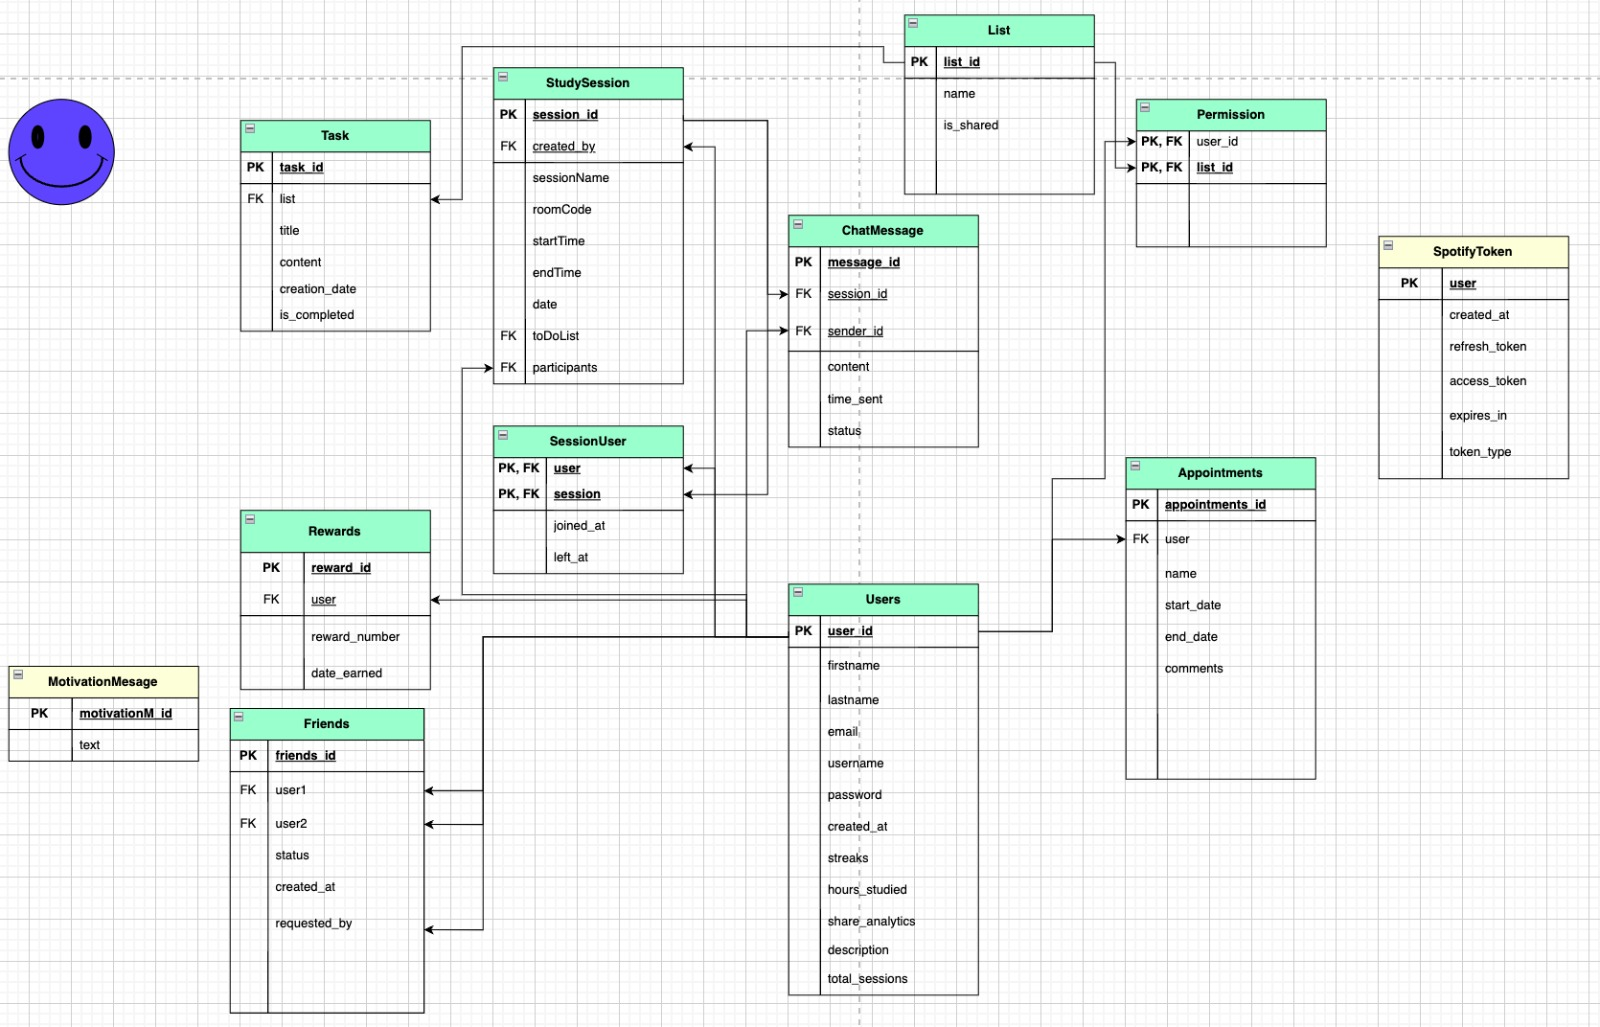
\includegraphics[width=1\linewidth]{ER-diagram.png}
    \caption{Finalised ER Diagram}
    \label{fig:er-diagram}
\end{figure}


\section{Implementation Details}
\label{sect:implementation-details}
\subsection{Initial Design Plan}
We gained inspiration from existing study group pages and the elements / components needed by the students. We brainstormed and mapped components onto paper: added components block-wise like a grid on the dashboard and group study pages. We used Figma to start designing how the UI components placement, colour scheme and overall presentation/layout of all the different pages: \textit{Login, Welcome Page, Dashboard, Group Study Room.}

\subsection{Finalised Features} Through the elimination process, we nailed down the ideas that reflected the goals of our project and made our idea unique. 
\begin{itemize}
    \item \textbf{To-Do List (shared):} This allows the user to create individual lists for themselves and separate group lists (when working as a group). 
    \item \textbf{Shared Materials:} Allows multiple users, in a group study session, to be able to share materials with each other in, but this is only active whilst the session is alive.
    \item \textbf{Timer:}This feature allows the user to schedule breaks within their desired focus time.
    \item \textbf{Chat box:} allowing users to communicate, while present in the group study room. This allows the user to be less distracted then on audio/video call, ensuring that communication is catered towards finishing the tasks.
    \item \textbf{Motivational Message:} These are randomly generated inspirational quotes, to encourage the user to continue studying and stay focused.
    \item \textbf{Profile Box:}  User can change their avatar (based on uploaded pictures from their device) and write a user description. This gives the user more creativity to customise their avatar and description to match them.
    \item \textbf{Statistics :} Collects data on the number of consecutive days they joined a study session (streaks) and also calculates the average time spent in the study room. This allows the user to track their time and remember to stay consistent with their studies. The user also has the option to share their data with friends, for some healthy competition. 
    \item \textbf{Friends List:} This allows the user to see the: friends list (which users they have accepted as friends), pending requests from new users, accepted friend requests and search for different friends. 
    \item \textbf{Calender:} This allows the user to schedule events, classes, exams and other assignment deadlines to keep up with and clearly organise a busy schedule.
    \item \textbf{Badges:} This is a type of reward system, that encourages the student to complete certain goals in order to achieve them. For instance, completing a certain number of hours, number of tasks etc.
    \item \textbf{Music: }Background music helps in productivity and makes the user feel more at ease when studying. It also helps avoid distraction and boosts motivation, each user independently listens to a track of their choice. Using Spotify API, premium users can control playback, helping to limit phone distraction.
    \item \textbf{Joined Users:} This allows the participants who are already in the room, to see who has joined.
    \item \textbf{Create/Join Room:} This allows user to create a study room/join a study room. This is the foundation of the project, which creates a platform for users to share learning materials, to-do list tasks, chat with each other, independently control timer and  music features.  And be inspired by the motivational messages. 

\end{itemize}

The \textbf{Welcome Page/Login/Sign Up} is simply designed to entice the user to login/sign up, using a vibrant pattern/colour scheme, is simplicity provides robust functionality to get the user seamlessly enter the platform.

\subsection{Dashboard and Group Study Page}
In both the \textbf{Dashboard} and \textbf{Group Study Page}, the components are arranged in columns. 

\begin{itemize}
    \item The \textbf{Dashboard} consists of: Profile Box, To-Do List, Join/Create Study Room, Friend Requests, Calendar, and Badges.
    \item The \textbf{Group Study Page} consists of: To-Do List, Shared Materials, Music, Joined Users, Motivational Message, Timer, and Chat Box.
\end{itemize}
 
This page has been tailored to the expectation of collaborative studies, where we have included the ability to exchange study materials with all users in the group, participate in educational conversations and create shared to do lists to complete with your team. 

There also additional features to help avoid distraction and boost maximum productivity with Timers, Music, Motivational quotes. 
The Group Study page includes a taskbar, to provide further functionalities to leave the group study room, copy-paste the room code, music feature and present the room code.

All these design decisions are reflected in the final product, the orientation of all these components has also been carefully crafted to meet the user's needs and expectations. Moreover, the layout has been slightly altered overtime to enhance user experience.



\section{Alternative Considerations}
\label{sect:alternative-considerations}
We researched and discussed several possibilities for different aspects of the project, from our tech stack to which features we should implement.

\subsection{Features}
Initially, we had planned to use an ChatGPT API to create small quizzes using the documents uploaded to the shared materials box in the group study room; however, we had to de-prioritise this feature due to lack of time, as well as us considering the other features to be of greater importance.

We also considered allowing users to join their friends' study rooms without a room code, i.e. implement a feature that lets you see which of your friends are currently online or in a study room, and being able to join them in that study room without needing to enter the room code. After much deliberation, we decided to put this feature on the back burner since users may not want their friends to be able to suddenly enter into a study room without their permission, particularly considering that most students have different study groups for different purposes and may not want members of one group mixing with another.


\subsection{Tech Stack}
We had decided on using Django for the backend of the project and React for the frontend quite early on in the timeline, however, it took us a while to settle on which database to use in order to store user data. In particular, we could not choose between SQLite and Firebase. 

Half of us wanted to stick to what we knew by using SQLite since that is what we used in the Small Group Project, whereas the other half wanted to learn something new and extend ourselves. In the end, we decided to use both; \begin{itemize}
    \item \textbf{Django Models} for structured data.
    \item \textbf{Firebase} for multimedia storage.
\end{itemize}

Our chosen architecture follows a modular and scalable approach, ensuring separation of concerns between the frontend, backend, and database. The React frontend provides a dynamic user experience and the Django backend was selected for its robustness in handling authentication, session management, and complex data processing. By using Firebase for multimedia storage, we had an option to provide real-time file sharing, which we would not have done with just the use of Django models. This architecture follows software engineering best practices such as scalability, maintainability, and modularity, ensuring that features can be expanded in future iterations without major restructuring.


\subsection{Deployment}
To ensure a swift and clean deployment, we planned and moved ahead with PythonAnywhere to deploy the backend (Django). Though this proved to be an oversight on our part as the free version of PythonAnywhere did not support websockets, which we had used in multiple features of the group study room - such as the chat and shared to-do list. After some further research and inquiring with other groups with a similar tech stack, we came to know about Render, which is what we finally used to deploy the backend.

Although we were unanimous in our decision for the backend deployment, the frontend deployment tools took slightly more time and effort. We looked into Azure, Cloudflare, Heroku, and a few other services, however they all did not have a free plan that met our needs. In the end, we came across Vercel and it seemed to meet all our requirements. It was very convenient to use Vercel since it is linked to our GitHub repository meaning it redeployed every time main is updated which means we do not have to dedicate extra time to deploying the frontend regularly.

\section{Changes During Development}
\label{sect:changes-during-development}

\subsection{Changes in UI Design}
The base design of the original UI utilised a limited range of colours and was slightly more flat in appearance, in addition to the repeated use of the black sans serif font. Our advisor suggested that we should ensure the UI was more cohesive, and that the study room component should be placed in the centre of the dashboard as it was our website’s unique selling point, as opposed to the profile component; consequently, we implemented this advice, and our profile box component was placed to the left. 
One of Onessa’s tasks was to ensure the UI flowed more and cultivated a more dynamic, inviting feel to the website. For the welcome page, her aim was to create a “mango” aesthetic true to the mango cat logo/ mascot of the website, utilising a range of reds and oranges for the upper and lower borders, with  mango emojis in the corner of the welcome box! This choice of bold and bright colours for the first page the users would see, intends to evoke a burst of energy and elation towards the notion of studying, which is universally seen as a boring task. 

The login and sign-up pages had more of a “peach” aesthetic with a range of pinks, yellows and light oranges. This would then transition into the “lighter” pink and blue aesthetic used for the dashboard, maintaining the same subtle and light colour theme throughout that was originally intended for the UI. Then it seamlessly morphs into the benevolent, rich deep purple and soft purple-blue colour schemes on the group study room page, to allow the room to feel immersive and inviting while also elevating user concentration. On this page the music, customisation, exit and copy code buttons were placed on the border as opposed to in the middle of the group study page where you can see the users in the room which was the case earlier, with the icons being buttons themselves as opposed to being on rounded buttons, as they are auxiliary to the room’s key components, and to ensure the central study area was less cluttered. 

The “Orbitron” font, with a subtle greyish shadow, was a unique choice that she used for the titles of each page in the borders; its geometric, futuristic style intends to motivate students to aim for the brightest future that they dream of having, which correlates with wanting to study/ focus more to achieve this. As for the other text on the pages, she kept the inter sans serif fonts but capitalised them and added subtle playful, pinkish shadows, accentuating the dynamic and cosy overall effect of the website. 

Finally, there was a smiley face slider that was originally going to be on the group study page but it was relocated to the analytics container on the dashboard, allowing the user to choose whether their friends could see their study statistics. This was an effective design choice; it ensured the dashboard was more streamlined while also enabling users to have more control over their privacy. 

\subsection{Changes in Implementation}
\textbf{Deployment Challenges} 

Upon first deployment to PythonAnywhere, a limitation we faced was that there was a paid tier for supporting Websockets, which a plethora of the key real-time features of our website relied upon. Thus, we mitigated by relocating the app to Vercel and Render, which possessed more scalable methods of hosting and real-time functionality, enabling us to achieve this for free. This uninterrupted, free inclusion of WebSockets fulfilled the technical and financial limitations of the project.

\textbf{Adapting Music Feature Integration for Accessibility}

The Spotify API used for the music component of the group study room possessed a large limitation, which we were initially unaware of. The reliance on Spotify Premium caused accessibility problems for users without this subscription. Hence, we transitioned to also integrating free music sources, giving us an availability of audio content; we were able to include a range of tracks that members of our group enjoyed, and as students ourselves, believed created the perfect ambience for studying as a group, from 2010 summer themed tracks to Pokemon and Animal Crossing tracks, adored by a range of students. From a user's standpoint, initially sticking to the Spotify Premium API may dissuade them from wanting to use the group study room if they frequently listen to music while studying and dislike ads, so the inclusivity incurred from this change was essential.

\textbf{User Authentication Workflow Refinements}

User authentication at first had issues with various accounts logged into the same browser using multiple tabs, resulting in token collision and unauthorised overriding, so only the most recently logged in user would be logged in on all tabs. We solved this by enforcing one active session per browser. However, lingering authentication cookies would sometimes prevent the user from logging in after partial sign-outs (for e.g, if the user lost connection, causing them to unintentionally log out). This was solved by implementing an automatic logout feature of all the user's logged in accounts triggered by them refreshing the page; this change was pivotal as it would encourage more consistent session management for the user.

\textbf{Evolution of the Calendar Feature}

The calendar feature, which started off as a feature that has a smaller preview on the dashboard and a large view when clicked on, evolved considerably during development. We replaced this preview with a streamlined calendar emoji button, reclaiming space on the interface for higher priority components. It also previously required manually changing the status of an event on the calendar to facilitate event colour coding, however that was optimised to be automatic given when the events took place: events in the past, present and future were represented with different colours. The feature's expansion points to how it has grown into a central tool for time management within the application, allowing users to visually prioritise tasks with more ease.

\section{Justification of Architectural Choices}
\label{sect:justification}
Our architecture follows software engineering best practices:
\begin{itemize}
    \item \textbf{Modularity:} Frontend (React), backend (Django), and database (Firebase/Django Models) are separated.
    \item \textbf{Scalability:} Features can be expanded without major restructuring.
    \item \textbf{Efficiency:} React ensures fast rendering, Django manages authentication, and Firebase handles real-time storage.
\end{itemize}
    \chapter{Testing}
\label{chap:testing}

\section{Testing Approach}
Our testing approach was a mix of unit testing, integration testing, and manual user testing. We aimed for high test coverage while keeping the process efficient and practical.

\begin{itemize}
    \item \textbf{Unit Testing:} We used Django’s built-in testing framework to cover backend logic and API endpoints, while Jest was used to test React components on the frontend.
    \item \textbf{Integration Testing:} WebSockets and API interactions were tested to ensure that real-time updates worked correctly.
    \item \textbf{User Testing:} We conducted manual user testing to validate the UI, interactions, and overall user experience.
\end{itemize}

We followed a test-as-you-go approach, meaning tests were written as soon as a feature was implemented. This helped us identify issues early rather than waiting until the end of development.

\subsection{Automated Tests}
Our automated tests included:

\begin{itemize}
    \item \textbf{Backend:} Django tests covered key functionalities, including authentication, WebSocket communication, and database operations.
    \item \textbf{Frontend:} Jest tests focused on user interface components, user interactions, and state updates.
    \item \textbf{End-to-End (E2E) Testing:} Some integration tests were performed manually, particularly for WebSocket-driven features in real time.
\end{itemize}

Currently, our test coverage stands at:
\begin{itemize}
    \item \textbf{Backend:} 93\%
    \item \textbf{Frontend:} 85\%
\end{itemize}

\textbf{Commands to Run Tests:}

\textbf{Backend (Django):}
\begin{verbatim}
python manage.py test
\end{verbatim}

\textbf{To generate a backend coverage report:}
\begin{verbatim}
coverage run manage.py test 
coverage report -m (or coverage html)
\end{verbatim}

\textbf{Frontend (React, Jest):}
\begin{verbatim}
npm test
\end{verbatim}

\textbf{To generate a frontend coverage report:}
\begin{verbatim}
npm test -- --coverage  (or npx test -- --coverage)
\end{verbatim}

\section{Manual Testing Appendix}
\label{sect:manual:testing}
\begin{itemize}
    \item WebSocket Real-Time Update
    \begin{itemize}
        \item \textbf{Test Steps:} Open two browser tabs, perform an action (send a message in the chatbox, upload a shared material, update the shared to-do list) in one, check if the updates reflect in the other.
        \item \textbf{Expected Outcome:} Updates should appear instantly in both tabs.
        \item \textbf{Last Performed:} 2025-03-26
        \item \textbf{Result:} Pass
    \end{itemize}

    \item UI Responsiveness
    \begin{itemize}
        \item \textbf{Test Steps:} Resize the window and check that all the components are still visible / usable on the page or can be scrolled to.
        \item \textbf{Expected Outcome:} UI should adjust properly for different window sizes.
        \item \textbf{Last Performed:} 2025-03-26
        \item \textbf{Result:} Pass
    \end{itemize}

    \item User Authentication and Toast Error Messages
    \begin{itemize}
        \item \textbf{Test Steps:} Attempt to login with correct and incorrect credentials
        \item \textbf{Expected Outcome:} Correct credentials should log in, incorrect should show a toast error.
        \item \textbf{Last Performed:} 2025-03-26
        \item \textbf{Result:} Pass
    \end{itemize}
\end{itemize}

\section{Quality assurance processes}
\label{sect:testing:process}
\textbf{1. Code Reviews}
    \begin{itemize}
        \item Every test written had to go through a quick review before it was push onto main, which made sure that tests were correctly implemented and efficient.
    \end{itemize}
\textbf{2. Meeting Minutes}
    \begin{itemize}
        \item Major testing decisions were documented in team meetings.
    \end{itemize}

\section{Evaluation of testing}
\label{sect:testing:evaluation}
\textbf{What Worked Well:}
\begin{itemize}
    \item \textbf{High test coverage:} With the 93\% back-end and 85\% front-end coverage, we achieved strong validation for most functionalities.
    \item \textbf{Early testing:} Writing tests alongside development helped us catch issues quickly.
    \item \textbf{Automated checks:} Tests helped prevent regressions before deployment.
\end{itemize}

\textbf{Challenges:}
\begin{itemize}
    \item \textbf{Test Maintenance:} One downside was that whenever we refactored React components to make them cleaner and more efficient, existing Jest tests often broke and had to be updated.
    \item \textbf{Real-time testing:} WebSocket features required manual testing in some cases, as automating real-time interactions can be complex.
\end{itemize}

\textbf{Conclusion:}  
Overall, our testing strategy gave us confidence in the reliability of the system. The main challenge was keeping frontend tests up-to-date during refactoring. In the future, we could improve this by using more snapshot testing and writing tests that are less dependent on specific component structures.
    % \chapter{Machine learning}
\label{chap:machine-learning}

\defaultInstructions

\begin{instructions}
By default, this chapter is not included in the report because most teams do \emph{not} need this chapter.  If your project requires this chapter, uncomment the \texttt{input} command that includes this chapter.
\end{instructions}

\begin{expectations}
If your project includes training a machine learning model, and you made an effort to evaluate alternative  approaches, teams should include this chapter discussing the machine learning work.  It is recommended to  include a short summary description for each considered approach, a clear description and rationale of the  approach taken to evaluate and compare the different algorithms, a table summarising the results obtained in evaluation, and your team's decision on what algorithm was chosen for incorporation in the system.  Also  explain how the team's results can be replicated.  This chapter is not required if an existing machine learning model or tool was used, or if the team did not evaluate the machine learning component.
\end{expectations}  % Uncomment this line if you need this chapter.

    \appendix
    % \chapter{Manual tests}
\label{chap:manual-tests}

\defaultInstructions

\begin{instructions}
By default, this chapter is not included in the report because many teams do \emph{not} need this chapter.  If your project requires this chapter, uncomment the \texttt{input} command that includes this chapter.
\end{instructions}

\begin{expectations}
If your team relied on manual testing, and the manual testing was carefully planned such that the team has a detailed written specification of its tests, then this chapter should be used to provide a list of all the team's tests.  A template table is provided to help format the tests.
\end{expectations}

\begin{longtable}{| p{.04\textwidth} | p{.40\textwidth} | p{.25\textwidth} | p{.18\textwidth} |} 
\hline
\# & Test script & Expected outcome & Outcome/date \\ \hline
\endhead
1 & Specify the actions the tester must undertake to run the test. & Specify what the tester must observe. &  \\ \hline
\end{longtable}  % Uncomment this line if you need this chapter.
\end{document}
